%# -*- coding: utf-8-unix -*-
%%==================================================
%% chapter07.tex
%%==================================================

%\bibliographystyle{sjtu2}%[此处用于每章都生产参考文献]
\chapter{系统测试和部署}
\label{chap:test_and_deploy}
本系统对重要的业务逻辑做了单元测试,对整个应用做了端对端测试,然后使用Solano CI做了持续集成,对于生产分支(也就是主分支,master branch),使用了AWS提供的code pipeline服务进行了自动部署。
\section{单元测试}
这里以Smart City模块的redux部分为例,即第\ref{chap:design_and_implement}章中图\ref{fig:redux_dir}所示的Redux文件夹,这一部分是典型的重要业务逻辑。测试主要针对Action Creators和SubReducers函数,在actions.test.js中主要是确保Action Creators会生成正确Action和 Async Action Creators会生成接收dispatch为参数的通用测试,asyncActions.test.js中是对Async Actions Creators的专项测试,各个文件夹中对于每个SubReducers也有对应的测试,确保SubReducers不会修改旧状态(previousState)而且返回正确的新状态(nextState)。

如代码\ref{lst:unit_test}所示,第一个测试检查了所有Action Types变量的值都等于自己的变量名,第二个测试检查了所有Action Types都有一个对于的普通Action Creator会返回这个类型的Action。如图\ref{fig:unit_test}所示,这是Smart City模块的单元测试结果。
\begin{lstlisting}[language={JavaScript}, label={lst:unit_test}, caption={单元测试样例代码}]
describe('redux actionCreators/', () => {
  // ...
  it('each action type\'s value is its name', () => {
    expect(normalActions).to.deep.equal(expectedNormalActionsKeys);
    actionTypes.forEach(actionTypeName => {
      expect(A[actionTypeName]).to.equal(actionTypeName);
    });
  });

  it('each actionType has a corresponding actionCreator returns this type of action', () => {
    expect(actionTypes.length === normalActions.length).to.be.true;
    actionTypes.forEach(actionTypeName => {
      const actionCreatorName = _.camelCase(A[actionTypeName]);
      expect(normalActions).to.include(actionCreatorName);
      expect(A[actionCreatorName]().type).to.equal(actionTypeName);
    });
  });
});
\end{lstlisting}

\begin{figure}[H]
 \centering
 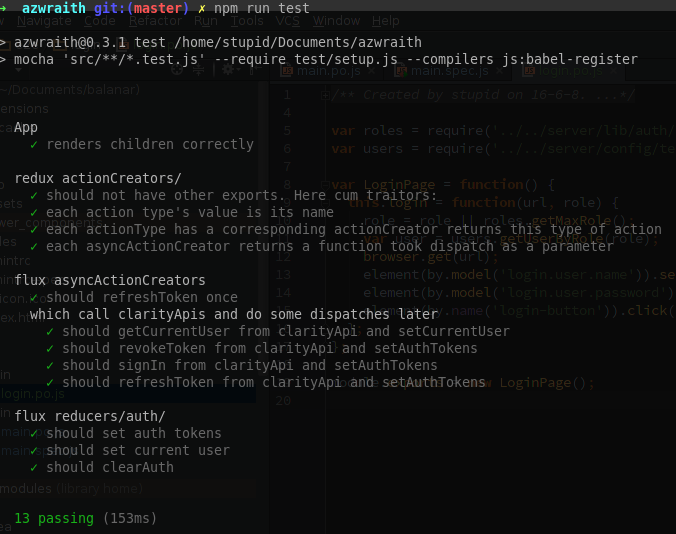
\includegraphics[width=0.8\textwidth]{azwraith_unit.png}
 \bicaption[fig:unit_test]{Smart City模块单元测试结果}{Smart City模块单元测试结果}{Fig}{Unit-test results of Smart City}
\end{figure}
\section{端对端测试}
执行端对端测试的过程中,Protractor会先启动服务器,然后自动打开chrome浏览器,在访问任何页面之前,先在登录页面自动填写用户名密码并提交,然后跳转到该页面。这里以版本管理模块的端对端测试为例,如代码\ref{lst:e2e_test}所示,该测试为了检查首页是否渲染成功在首页上检查了三个小标题中的问题内容是否正确。。如图\ref{fig:e2e_test}所示,这是版本管理模块端对端测试的命令行结果。
\begin{lstlisting}[language={JavaScript}, label={lst:e2e_test}, caption={端对端测试样例代码}]
/* 在login/login.po.js中 */
var LoginPage = function() {
  this.login = function(url, role) {
    role = role || roles.getMaxRole();
    var user = users.getUserByRole(role);
    browser.get(url);
    element(by.model('login.user.name')).sendKeys(user.name);
    element(by.model('login.user.password')).sendKeys(user.password);
    element(by.name('login-button')).click();
  };
};

/* 在main/main.spec.js中 */
describe('Main View', function() {
  var page;

  beforeEach(function() {
    var loginPage = require('../login/login.po');
    loginPage.login('/');
    page = require('./main.po');
  });

  it('should include jumbotron with correct data', function() {
    page.content.all(by.tagName('h2')).then(function(headers) {
      expect(headers.length).toBe(3);
      expect(headers[0].getText()).toBe('Designed a new component?');
      expect(headers[1].getText()).toBe('Ordered a new batch?');
      expect(headers[2].getText()).toBe('Assembled new sensors?');
    });
  });
});
\end{lstlisting}

\begin{figure}[!htp]
 \centering
 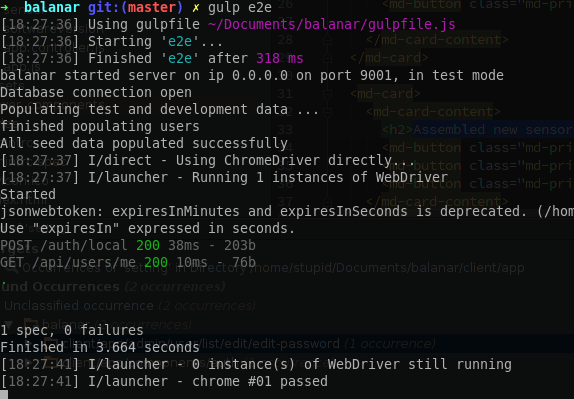
\includegraphics[width=0.8\textwidth]{balanar_e2e.png}
 \bicaption[fig:e2e_test]{版本管理模块端对端测试结果}{版本管理模块端对端测试结果}{Fig}{E2E-test results of Version Management}
\end{figure}

\section{自动部署}
AWS的CodePipeline提供的自动部署一般分为三个步骤,分别是从在线版本管理系统获取新版本的代码,编译代码,然后运行编译结果,在本系统中在线版本管理系统是Github,编译代码部分交给持续集成,最后用Node运行持续集成提交上来的结果。这里以版本管理模块的自动部署为例,如图\ref{fig:code_pipeline}所示这是在AWS上配置了三个步骤的自动部署流程。
\begin{figure}[H]
 \centering
 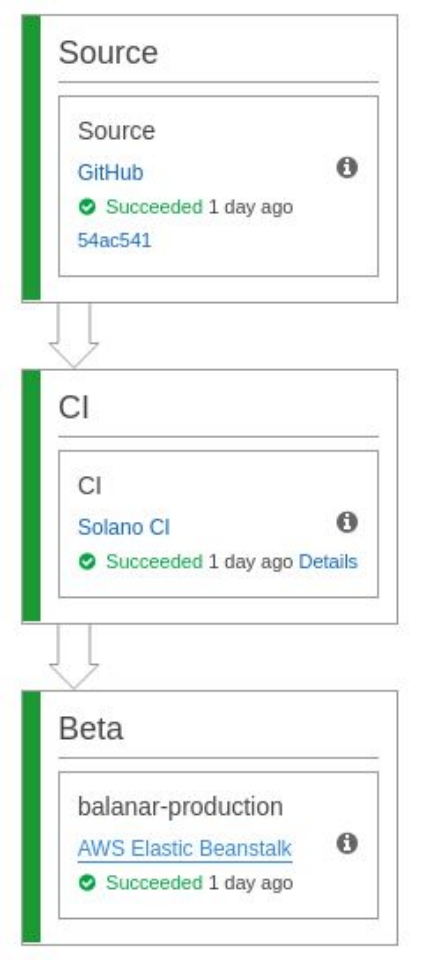
\includegraphics[width=0.4\textwidth]{code_pipeline.jpg}
 \bicaption[fig:code_pipeline]{版本管理模块自动部署流程}{版本管理模块自动部署流程}{Fig}{Code pipeline of Version Management}
\end{figure}

\section{持续集成}
SolanoCI简单的持续集成只需要一个solano.yml配置文件放在项目根目录下面就行了,本系统因为要和AWS的自动部署配合,所以需要在持续集成时进行编译,所以额外使用了一些脚本在solano.yml中调用。这里以Smart City模块的持续集成配置为例,介绍本系统的持续集成情况,该模块因为使用了ES6需要用NodeJS5来编译,而AWS上面只提供了NodeJS4的运行环境,所以持续集成时涉及到多个Node版本的切换,使用了一个叫nvm的库来切换Node版本。如代码\ref{lst:azwraith_ci}所示,持续集成时分2个任务(tests),分别确保进行编译和测试的完成,另有一些钩子(hooks)分布在持续集成的生命周期中:
\begin{description}
  \item[pre-setup] 在启动持续集成之前下载安装nvm并且提前安装好要用的Node4和Node5,最后用Node5安装了执行任务所需要的依赖
  \item[tests] 各个任务会在pre-setup之后post-worker之前执行。
  \item[post-worker] 在每个任务完成后,执行用于发布(--release)的编译(npm run build),并在编译的结果中,使用Node4来安装(npm install)生产环境(--production)的依赖,然后把build文件夹打包并复制到一个特殊的文件夹,SolanoCI之后会把这个文件夹中的内容作为持续集成中这一步的结果上传到服务器上,这样本模块的开发人员就可以下载到持续集成时产生的编译结果,出现错误时方便调试。
  \item[post-build] 在所有任务完成之后,用build文件夹代替了当前文件夹,因为AWS最后会把这个目录作为编译结果。
\end{description}

\begin{lstlisting}[language={JavaScript}, label={lst:azwraith_ci}, caption={Smart City模块持续集成配置}]
hooks:
  pre_setup: bash ./tools/solano/pre-setup.sh
  post_worker: bash ./tools/solano/post-worker.sh
  post_build: bash ./tools/solano/post-build.sh
test_pattern: 'none'
nodejs: false
iojs: false
tests:
  - source ./tools/solano/load-nvm.sh && nvm use 5 && npm run build
  - source ./tools/solano/load-nvm.sh && nvm use 5 && npm test

# pre-setup.sh
curl -o- https://raw.githubusercontent.com/creationix/nvm/v0.31.0/install.sh | bash
source ./tools/solano/load-nvm.sh
nvm install 4
npm install -g npm@3
nvm install 5

npm install

# post-worker.sh
source ./tools/solano/load-nvm.sh
nvm use 5

npm run build -- --release

nvm use 4
(cd build && npm install --production)
(cd build && zip -qr ../build.zip .)
cp build.zip $HOME/results/$TDDIUM_SESSION_ID/session/

# post-build.sh
mv build ../
dir=$(pwd -P)
cd ..
rm -rf -- "$dir"
mv build "$dir"
cd "$dir"
\end{lstlisting}

一个SolanoCI的项目会自动监控对应项目的所有分支,不过有自动部署的master分支会由AWS的Code Pipeline来触发持续集成,所以在SolanoCI的配置页面中去掉了master分支。如图\ref{fig:solano}所示,eb开头的持续集成时由AWS的Elastic Beanstalk触发的,dashboard对应的就是azwraith项目的生产环境,普通分支的持续集成时SolanoCI自己触发的。
\begin{figure}[!htp]
 \centering
 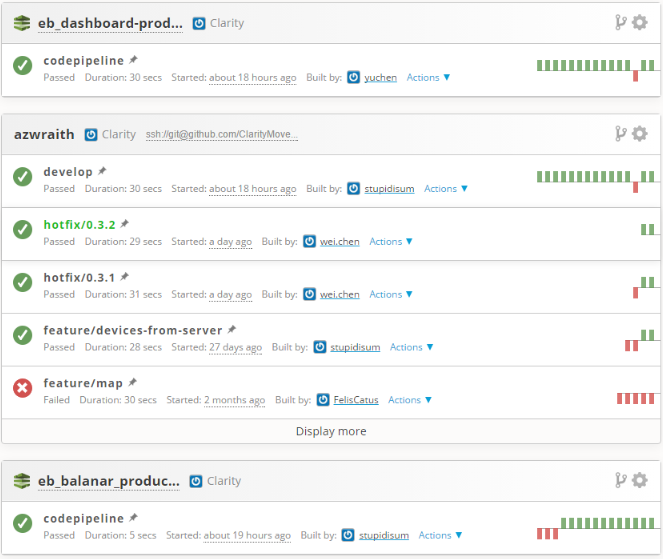
\includegraphics[width=\textwidth]{solano.png}
 \bicaption[fig:solano]{本系统在SolanoCI的持续集成页面}{本系统在SolanoCI的持续集成页面}{Fig}{Dashboard of SolanoCI}
\end{figure}

